\chapter{Development of Algorithms and Methodologies}
\label{sec:3}

\section{Datasets}
\label{sec:datasets}

\subsection{MobiFall v2.0 -- Human Fall Dataset}

The MobiFall v2.0 dataset \citep{mobifall2024} contains 6-axis IMU recordings (3-axis accelerometer and 3-axis gyroscope) collected from 24 human subjects performing both fall and Activities of Daily Living (ADL). Recordings were made with a smartphone placed in the trouser pocket, sampled at 50 Hz. The dataset provides recordings for nine fall types (forward fall, backward fall, lateral fall, etc.) and nine ADL types (walking, jogging, sitting, stairs, etc.).

Preprocessing extracts subject identifiers from filenames to support subject-independent train/test splits. Each subject's data is segmented into 128-sample windows with a 50\% step overlap (64 samples), yielding a final dataset of approximately 5,000 labelled windows (Fall or Normal).

\subsection{Physics-Based Synthetic Crash Dataset}

No publicly available labeled real-world crash dataset exists for smartphone IMUs. To overcome this, a physics-based crash generator was developed (\url{scripts/generate_car_crash_data.py}). The generator simulates two types of sequences:

\begin{itemize}
    \item \textbf{Crash sequences}: A pre-crash velocity phase, a high-G deceleration spike (20--50 g over 50--150 ms), and a post-crash silence with small gravity residual. The post-crash resting orientation matrix $\mathbf{R}_{\text{rest}}$ is randomised so the model learns orientation-invariant features.
    \item \textbf{Normal driving sequences}: Slow vehicle motion with small acceleration variations, mild cornering, and braking below the crash threshold.
\end{itemize}

The generator produced 200 crash and 200 normal sequences, each 128 samples at 50 Hz, for a total dataset of 400 windows. This matches the NHTSA crash test standard of 20--40 g peak deceleration for typical frontal collisions.

\section{System Architecture}
\label{sec:architecture}

The complete system follows the pipeline shown in Figure~\ref{fig:architecture}.

\begin{figure}[!h]
    \centering
    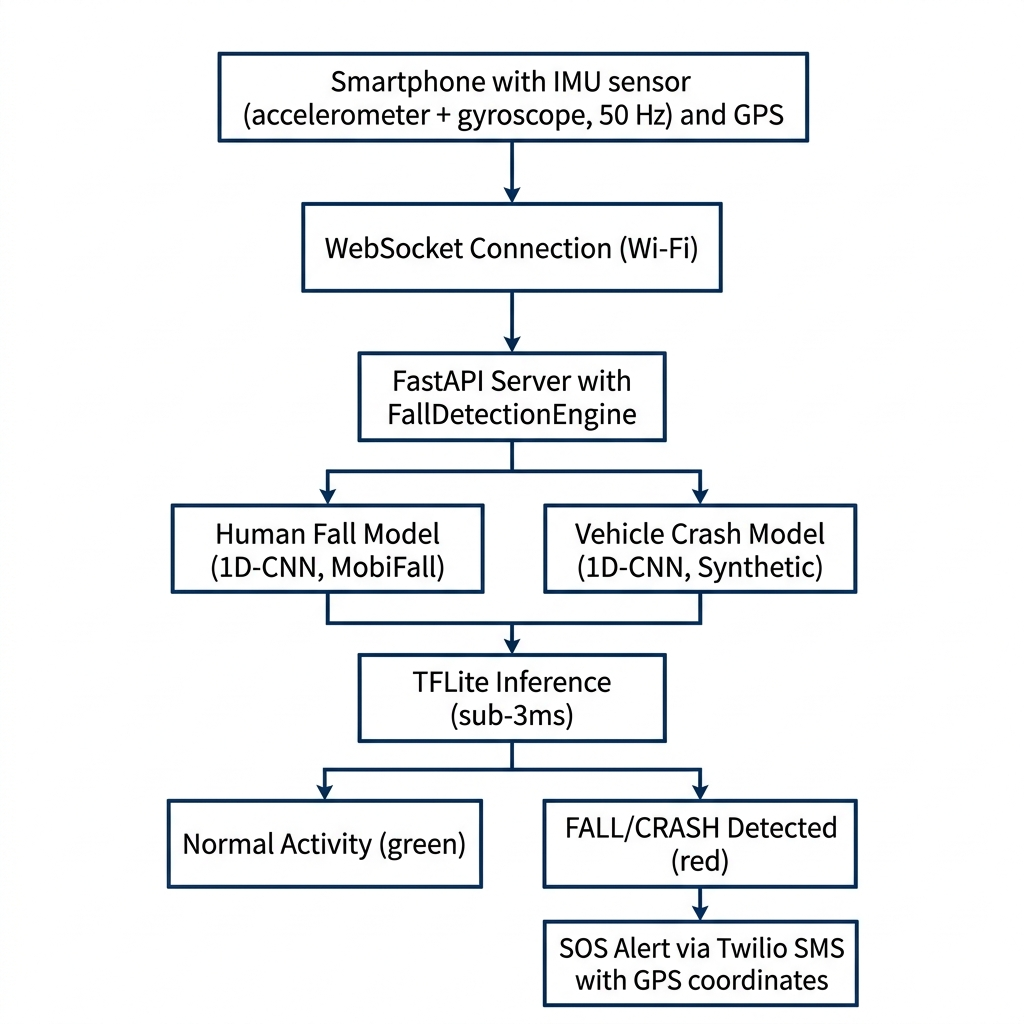
\includegraphics[width=0.85\textwidth]{images/system_block_diagram.png}
    \caption{High-level system architecture showing the data flow from smartphone IMU through the WebSocket server, inference engine, and Twilio SOS alerting.}
    \label{fig:architecture}
\end{figure}

\subsection{Mobile Dashboard (Frontend)}

An HTML5 dashboard running in the mobile browser requests \texttt{DeviceMotionEvent} permission and streams raw accelerometer and gyroscope readings to the FastAPI server over a persistent WebSocket connection at 50 Hz. Each message is a 6-key JSON object:
\begin{equation}
    \mathbf{s}_t = \{a_x, a_y, a_z, g_x, g_y, g_z\}
    \label{eq:sensor_sample}
\end{equation}
The dashboard also reads GPS coordinates and current speed via the Geolocation API and includes these in the crash alert payload.

\subsection{FastAPI WebSocket Server}

The server (\texttt{src/app.py}) is built with FastAPI and served by Uvicorn. It exposes the following endpoints:
\begin{itemize}
    \item \texttt{WebSocket /ws/predict} -- Accepts the 50 Hz sensor stream, passes each sample to \textit{FallDetectionEngine}, and returns predictions.
    \item \texttt{GET /health} -- Returns engine statistics (model loaded, total inferences, fall count).
    \item \texttt{POST /predict/single} -- REST alternative for single-sample push inference.
    \item \texttt{POST /switch-model} -- Hot-swaps the active model between human fall and crash mode.
\end{itemize}

\subsection{FallDetectionEngine -- Inference Engine}

The core inference engine (\texttt{src/inference.py}) maintains a circular deque buffer of size $W = 128$ samples. On each incoming sample, the engine appends to the buffer and increments a step counter. When the buffer is full and the step counter reaches the step size $S = 64$, it:
\begin{enumerate}
    \item Converts the buffer to a NumPy array of shape $(W, 6)$.
    \item Normalises the window using the training-set mean and standard deviation.
    \item Invokes the TFLite interpreter.
    \item Applies a static guardrail: if the acceleration magnitude variance falls below $\sigma^2_{\text{thresh}} = 0.05$, the output is overridden to ``Normal'' regardless of the raw model score.
    \item Returns the label, confidence score, and inference latency.
\end{enumerate}

The engine holds a dictionary of two TFLite interpreters (``human'' and ``car'') and switches between them atomically, making hot-swapping thread-safe.

\section{Model Architectures}
\label{sec:models}

\subsection{1D-CNN (Selected Architecture)}

The deployed model is a one-dimensional convolutional network. Its structure is:

\begin{itemize}
    \item \textbf{Input}: $(128, 6)$ -- 128 timesteps, 6 IMU channels.
    \item \textbf{Conv1D (64 filters, kernel 3, ReLU)} + BatchNormalization + MaxPooling1D (2).
    \item \textbf{Conv1D (128 filters, kernel 3, ReLU)} + BatchNormalization + MaxPooling1D (2).
    \item \textbf{GlobalAveragePooling1D}.
    \item \textbf{Dense (64, ReLU)} + Dropout (0.5).
    \item \textbf{Dense (1, Sigmoid)} -- binary output (Fall / Normal).
\end{itemize}

Total trainable parameters: \textbf{8,481}. After TFLite dynamic quantization, the model occupies approximately \textbf{15 KB}.

\subsection{Compared Architectures}

Three additional architectures were implemented and evaluated on identical training conditions:
\begin{itemize}
    \item \textbf{LSTM}: Two stacked LSTM layers (64 units each) followed by a Dense sigmoid output. 20,289 parameters.
    \item \textbf{CNN-LSTM}: Two Conv1D layers feeding into an LSTM layer. 36,353 parameters.
    \item \textbf{Transformer}: A single multi-head self-attention block (2 heads) with a dense projection, no positional encoding. 1,557 parameters.
\end{itemize}

\section{Training Protocol}
\label{sec:training}

All models were trained using the following protocol:
\begin{itemize}
    \item \textbf{Optimiser}: Adam, learning rate = 0.001.
    \item \textbf{Loss}: Binary cross-entropy.
    \item \textbf{Batch size}: 64.
    \item \textbf{Epochs}: Up to 10, with EarlyStopping (patience = 3) monitoring validation loss.
    \item \textbf{Checkpoint}: ModelCheckpoint saves the best-validation-loss weights.
    \item \textbf{Split}: 80\% train / 20\% test, stratified by class.
\end{itemize}

A 5-fold cross-validation was also performed on the crash dataset to confirm stability of the result.

\section{TFLite Quantization and Edge Deployment}
\label{sec:deployment_method}

The trained Keras \texttt{.h5} model is converted to TFLite using \url{src/tflite_converter.py}:

\begin{lstlisting}[language=Python, caption={TFLite conversion with dynamic range quantization.}]
converter = tf.lite.TFLiteConverter.from_keras_model(model)
converter.optimizations = [tf.lite.Optimize.DEFAULT]
tflite_model = converter.convert()
with open("models/mobifall_edge_model.tflite", "wb") as f:
    f.write(tflite_model)
\end{lstlisting}

Dynamic quantization converts 32-bit float weights to 8-bit integers, reducing the model from 140 KB to approximately 15 KB -- an 89\% reduction -- with negligible accuracy loss. At runtime the engine auto-detects whether the full \url{tensorflow} package or the lightweight \url{tflite_runtime} is available, enabling transparent deployment on both development machines and Raspberry Pi.

\section{SOS Alert System}
\label{sec:sos}

On crash detection at speed above a configurable threshold, the \texttt{notifier.py} module constructs an SMS containing:
\begin{itemize}
    \item GPS latitude and longitude (from the browser Geolocation API).
    \item Last known vehicle speed.
    \item Detection confidence and timestamp.
\end{itemize}
The message is dispatched via the Twilio REST API to one or more pre-configured emergency contact numbers. If Twilio credentials are absent, the notifier falls back to a mock alert printed to the server log.